\documentclass[11pt]{article}
\usepackage[utf8]{inputenc}
\usepackage{polski} 
\usepackage{geometry}
\geometry{a4paper}
\usepackage{graphicx}
\usepackage{booktabs}
\usepackage{array}
\usepackage{paralist}
\usepackage{verbatim}
\usepackage{subfig}
\usepackage{amsmath}
\usepackage{float}
\usepackage{amsthm}
\usepackage{amssymb}
\usepackage{amsfonts}
\usepackage{float}
\usepackage{thmtools}
\theoremstyle{definition}
\newtheorem{zad}{Zadanie}
\numberwithin{zad}{section}
\newtheorem{theorem}{Twierdzenie}
\newtheorem{definition}{Definicja}
\newtheorem{lemma}{Lemat}
\renewcommand*{\proofname}{Rozwiązanie}

\usepackage{fancyhdr}
\pagestyle{fancy}
\renewcommand{\headrulewidth}{0pt}
\usepackage{sectsty}
\allsectionsfont{\sffamily\mdseries\upshape}
\usepackage[nottoc,notlof,notlot]{tocbibind}
\usepackage[titles,subfigure]{tocloft}
\renewcommand{\cftsecfont}{\rmfamily\mdseries\upshape}
\renewcommand{\cftsecpagefont}{\rmfamily\mdseries\upshape}
\newcommand{\blank}{\framebox{\phantom{xxx}} }
\title{Fizyka}

\begin{document}
\maketitle
\tableofcontents

\section{Kinematyka}

\subsection{Prędkość, droga, czas}

Zrobimy głównie zadania matematyczne.

\begin{figure}[H]
\centering

\includegraphics[width=0.8\linewidth]{./svt/zad1.png}
\end{figure}
\begin{figure}[H]
\centering

\includegraphics[width=0.8\linewidth]{./svt/zad2.png}
\end{figure}
\begin{figure}[H]
\centering
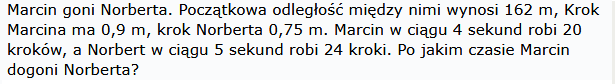
\includegraphics[width=0.8\linewidth]{./svt/zad3.png}
\end{figure}
\begin{figure}[H]
\centering
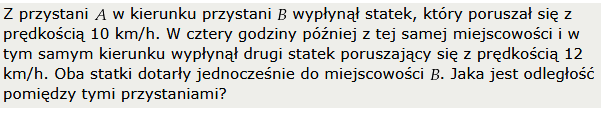
\includegraphics[width=0.8\linewidth]{./svt/zad4.png}
\end{figure}
\begin{figure}[H]
\centering
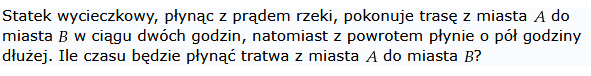
\includegraphics[width=0.8\linewidth]{./svt/zad5.png}
\end{figure}
\begin{figure}[H]
\centering
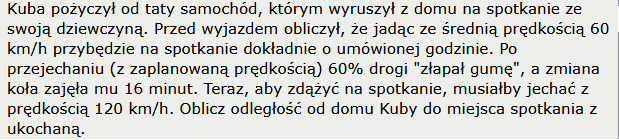
\includegraphics[width=0.8\linewidth]{./svt/zad6.png}
\end{figure}

\begin{figure}[H]
\centering
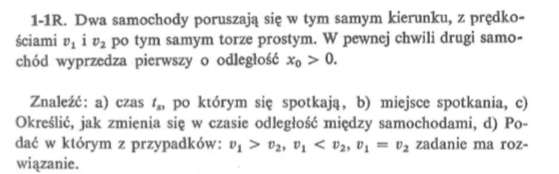
\includegraphics[width=0.8\linewidth]{./svt/kruczek1.png}
\end{figure}

\begin{figure}[H]
\centering
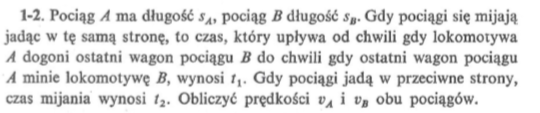
\includegraphics[width=0.8\linewidth]{./svt/kruczek2.png}
\end{figure}

\begin{figure}[H]
\centering
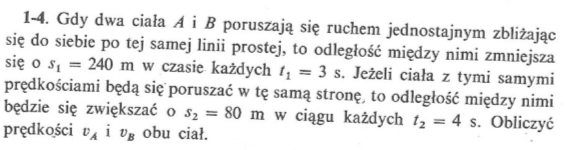
\includegraphics[width=0.8\linewidth]{./svt/kruczek3.png}
\end{figure}

\begin{figure}[H]
\centering
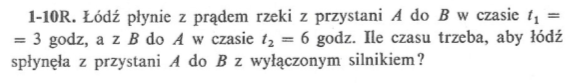
\includegraphics[width=0.8\linewidth]{./svt/kruczek4.png}
\end{figure}

\section{Dynamika}
\subsection{Zasady dynamiki Newtona}

Zacznijmy od wymienienia wszystkich trzech zasad:

\begin{enumerate}
\item Ciało na którą działa zerowa siła wypadkowa porusza się bez przyspieszeń.
\item Przyspieszenie ciała jest wprost proporcjonalne do wypadkowej siły nań działającej.
\item Oddziaływania ciał są zawsze wzajemne. Suma oddziaływań w układach inercjalnych zawsze się zeruje.
\end{enumerate}

\subsection{Rodzaje oddziaływań}

Nowoczesna fizyka rozróżnia cztery podstawowe oddziaływania:

\begin{enumerate}
\item Grawitacja,
\item Elektromagnetyzm,
\item Oddziaływania silne,
\item Oddziaływania słabe.
\end{enumerate}

Ostatnie dwa odpowiadają za oddziaływania wewnątrz atomowe - dzięki oddziaływaniom silnym kwarki trzymają się razem i tworzą neutrony i protony, które następnie tworzą jądra atomów. Oddziaływania słabe są znacznie bardziej subtelne i występują w przemianach kwarków i leptonów. Dwa pierwsze oddziaływania znamy znacznie lepiej z życia - grawitacja jest oddziaływaniem mas na siebie, elektromagnetyzm jest oddziaływaniem ładunków elektrycznych na siebie.

\subsection{...inne oddziaływania?}

Na lekcjach fizyki poznamy inne siły - siłę tarcia, siłę oporu, siłę wyporu, siłę sprężystości, etc etc. Nie są to manifestacje nowych oddziaływań, tylko doświadczalne przejawy znanych efektów.

\section{Zadania z fizyki}

\begin{zad}
Jaką siłę należy nadać kulce o masie 0.5 kg aby poruszała się z przyspieszeniem 2 $\frac m{s^2}$?
\end{zad}

\begin{zad}
Ciało o masie 2 kg porusza się  z przyspieszeniem 5 $\frac m{s^2}$. Oblicz wartość działającej siły.
\end{zad}

\begin{zad}
Na obiekt o masie 5 kg działamy siłą 20 N. Jednocześnie na obiekt działa siła tarcia o wartości 5 N. Oblicz przyspieszenie z jakim porusza się ciało.
\end{zad}

\begin{zad}
Ciało o masie 10 kg podlega oddziaływaniu siły o wartości 50 N. Na ciało działa również siła tarcia. Obiekt porusza się z przyspieszeniem 2 $\frac m{s^2}$. Oblicz wartość siły tarcia.
\end{zad}

\begin{zad}
Na ciało działa siła 30 N oraz siła tarcia wartości 20 N. Ciało porusza się z przyspieszeniem 20 $\frac m{s^2}$. Oblicz masę ciała.
\end{zad}

\begin{zad}
Ciało o masie 5 kg porusza się po poziomej powierzchni o współczynniku tarcia $k = 5$. Równanie określające zależność siły tarcia od siły nacisku jest dane jako:

$$F_t = kN,$$

gdzie $F_t$ to wartość siły tarcia, $k$ to współczynnik tarcia, a $N$ to wartość siły nacisku. Nacisk na poziomą powierzchnię jest równy wartości siły ciężkości (ciężaru) ciała, równej

$$F_c = mg,$$

gdzie $g$ oznacza przyspieszenie ziemskie. Znajdź przyspieszenie ciała, jeśli działamy na nie siłą o wartości 20 N.
\end{zad}

\begin{zad}
Jak będzie się różniło rozwiązanie poprzedniego zadania, jeśli zamiast na powierzchni Ziemi przeprowadzimy eksperyment na powierzchni a) Księżyca, b) Marsa, c) Saturna.

\begin{figure}[h]
\centering
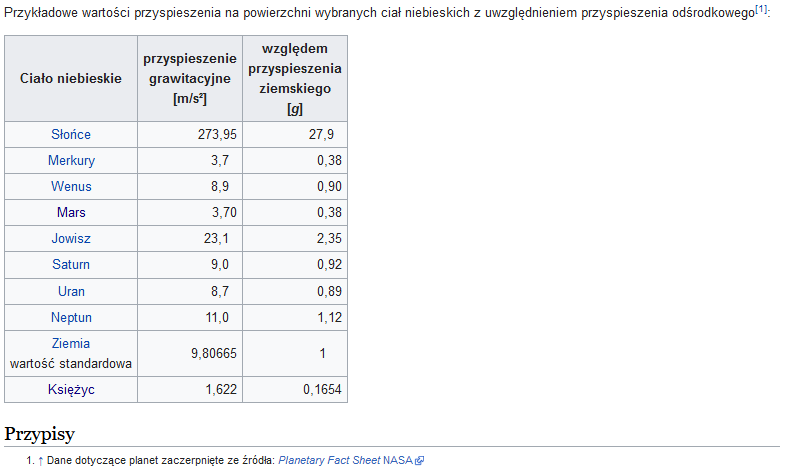
\includegraphics[width=1\linewidth]{przyspieszenia.png}
\end{figure}
\end{zad}

\begin{zad}
Jaki dystans przeleci ciało w ciągu 5 sekund, jeśli porusza się z przyspieszeniem 10 $\frac{m}{s^2}$ i zaczyna ruch z zerową prędkością?
\end{zad}

\begin{zad}
Ciało porusza się z przyspieszeniem 7 $\frac m{s^2}$. W ciągu 2 sekund obiekt pokonał drogę o długości 20 m. Oblicz jaka była prędkość początkowa ciała.
\end{zad}

\begin{zad}
Obiekt porusza się z przyspieszeniem $a=5 \frac ms$ i zerową prędkością początkową. Oblicz, ile czasu potrzebuje na pokonanie dystansu 40 m.
\end{zad}

\subsection{Energia}

Wzór na energię kinetyczną:

\begin{equation}
E_k = \frac{mv^2}2.
\end{equation}

Wzór na energię potencjalną:

\begin{equation}
E_p = mgh.
\end{equation}

Jednostka energii: dżul [J]. $1 J = 1 N \cdot 1 m = \frac{kg \cdot m^2}{s^2}.$

\begin{zad}
Oblicz energię kinetyczną ciała o masie 2 kg i prędkości $5 \frac ms$.
\end{zad}

\begin{zad}
Jaką masę musi mieć ciało poruszające się z prędkością $3 \frac ms$, aby jego energia kinetyczna wynosiła 45 J?
\end{zad}

\begin{zad}
Z jaką prędkością musi poruszać się obiekt o masie 5 kg aby jego energia kinetyczna wynosiła 10 J?
\end{zad}

\begin{zad}
Ciało o masie 5 kg porusza się z przyspieszeniem 10 $\frac m{s^2}$. Jaką energię kinetyczną będzie miało po 10 sekundach?
\end{zad}

\begin{zad}
Jeśli ciało zostanie rzucone w górę, energia kinetyczna będzie stopniowo przechodziła w energię potencjalną podczas wznoszenia się ciała ku górze, w końcu wytracając całą energię kinetyczną będąc przez chwilę nieruchome na szczycie trasy. Następnie ciało zacznie opadać, ponownie przekształcając energię potencjalną w kinetyczną podczas wytracania wysokości.

Przez cały czas suma energii pozostanie stała:

\begin{equation}
E_k + E_p = const.
\end{equation}

Oblicz na jaką wysokość wzniesie się ciało o masie 2 kg, jeśli zostało rzucone ku górze z energią kinetyczną równą 20 J.
\end{zad}

\begin{zad}
Oblicz na jaką wysokość poleci ciało o masie 1 kg, jeśli zostało rzucone z prędkością 20 $\frac ms$. Czy znajomość masy była potrzebna?
\end{zad}

\end{document}
